\documentclass[conference]{IEEEtran}
\IEEEoverridecommandlockouts
\usepackage[utf8]{inputenc}
\usepackage[T1]{fontenc}
\usepackage[brazil]{babel}
\usepackage{cite}
\usepackage{amsmath,amssymb,amsfonts}
\usepackage{algorithmic}
\usepackage{graphicx}
\usepackage{textcomp}
\usepackage{xcolor}
\usepackage{booktabs}
\usepackage{placeins}
\usepackage{float}
\def\BibTeX{{\rm B\kern-.05em{\sc i\kern-.025em b}\kern-.08em
    T\kern-.1667em\lower.7ex\hbox{E}\kern-.125emX}}
\begin{document}

\title{Embeddings de not\'icias financeiras e comunicados do Copom em portugu\^es na previs\~ao do retorno di\'ario do Ibovespa: uma avalia\c{c}\~ao com valida\c{c}\~ao walk-forward}

\author{\IEEEauthorblockN{Hiago Lacerda}
\IEEEauthorblockA{\textit{Deep Learning} \\
\textit{Universidade Federal de Pernambuco - UFPE}\\
Recife, Brasil \\
hwal@cin.ufpe.br}
}

\maketitle

\begin{abstract}
Este trabalho avalia se embeddings textuais de not\'icias financeiras e o sinal de pol\'itica monet\'aria do Copom, ambos em portugu\^es, melhoram a previs\~ao do retorno di\'ario (D+1) do Ibovespa frente a baselines cl\'assicos (passeio aleat\'orio, ARIMA/ARIMAX) e a um modelo tabular treinado s\'o com pre\c{c}o (XGBoost). Manchetes do InfoMoney (2018--2024, 57.611 registros) foram convertidas em embeddings por BERTimbau e FinBERT-PT-BR e combinadas a uma LSTM parcimoniosa treinada sobre vari\'aveis de pre\c{c}o, sob protocolo walk-forward com embargo de 21 dias e ajuste de todo componente dependente de dados exclusivamente no treino de cada fold. Nenhum modelo supera o acaso na previs\~ao direcional de forma estatisticamente significativa (Pesaran-Timmermann, $p>0{,}05$ ap\'os Holm em todos os casos). O sinal textual \'e reativo, n\~ao preditivo: a polaridade de sentimento correlaciona-se com o retorno do mesmo dia ($r\approx0{,}20$), mas n\~ao com o de D+1 ($r$ entre $0{,}00$ e $-0{,}04$). Testes de Diebold-Mariano mostram que o XGBoost \'e significativamente mais preciso do que diversas variantes de LSTM com texto, nunca o inverso. Sob custo de 5 bps/opera\c{c}\~ao, dez das onze estrat\'egias mec\^anicas t\^em Sharpe negativo ou nulo; a exce\c{c}\~ao \'e indistingu\'ivel de zero e inst\'avel entre folds. Uma verifica\c{c}\~ao de robustez, retreinando os modelos sobre o corpo completo das mat\'erias (56.819 textos, n\~ao apenas a manchete), reproduz o mesmo padr\~ao nulo. Conclui-se que, sob valida\c{c}\~ao rigorosa e sem vazamento temporal, embeddings de not\'icias financeiras em portugu\^es n\~ao melhoram a previs\~ao do retorno di\'ario do Ibovespa -- resultado nulo obtido com rigor metodol\'ogico, n\~ao uma limita\c{c}\~ao de implementa\c{c}\~ao.
\end{abstract}

\begin{IEEEkeywords}
previs\~ao de s\'eries financeiras, embeddings de texto, BERTimbau, FinBERT, valida\c{c}\~ao walk-forward, Ibovespa
\end{IEEEkeywords}

\section{Introdu\c{c}\~ao}

A hip\'otese de que not\'icias financeiras carregam informa\c{c}\~ao capaz de antecipar movimentos de pre\c{c}o \'e conhecida na literatura de finan\c{c}as e ganhou renovado interesse com modelos de linguagem baseados em Transformers, que tornaram vi\'avel extrair representa\c{c}\~oes vetoriais densas de texto em portugu\^es sem depender de l\'exicos de sentimento curados manualmente. Este trabalho investiga se embeddings textuais em portugu\^es, extra\'idos de not\'icias financeiras, melhoram a previs\~ao do retorno di\'ario (D+1) do Ibovespa frente a baselines financeiros cl\'assicos e a um modelo tabular robusto treinado apenas com pre\c{c}o.

O desenho experimental adota uma progress\~ao incremental de complexidade -- passeio aleat\'orio, ARIMA/ARIMAX, XGBoost, LSTM s\'o com pre\c{c}o, LSTM com texto ou sinal do Copom --, na qual cada n\'ivel \'e validado isoladamente antes de servir de refer\^encia ao seguinte: um ganho real de texto deve superar o melhor modelo de pre\c{c}o j\'a constru\'ido, n\~ao apenas um baseline artificialmente fraco.

O alvo de todos os modelos \'e o log-retorno de D+1,
\begin{equation}
y_t = \ln\!\left(\frac{\text{close}_{t+1}}{\text{close}_t}\right),
\label{eq:target}
\end{equation}
avaliado por magnitude do erro (MAE, RMSE), acerto direcional (DA, F1, MCC) e calibra\c{c}\~ao (Brier). A valida\c{c}\~ao segue sempre esquema walk-forward temporal, com toda transforma\c{c}\~ao dependente dos dados -- normaliza\c{c}\~ao, PCA, calibra\c{c}\~ao, sele\c{c}\~ao de ordem ARIMA -- ajustada exclusivamente no treino de cada fold.

Contribui\c{c}\~oes deste trabalho:
\begin{itemize}
\item Corpus de 57.611 manchetes do InfoMoney (2018--2024) com atribui\c{c}\~ao temporal por corte \`as 17h, incluindo hor\'ario de ver\~ao hist\'orico.
\item Compara\c{c}\~ao sim\'etrica entre BERTimbau e FinBERT-PT-BR, embeddings e sentimento expl\'icito.
\item Evid\^encia de que o sinal textual \'e reativo, n\~ao preditivo (Se\c{c}\~ao~\ref{sec:achado}).
\item Protocolo estat\'istico abrangente (Diebold-Mariano, Pesaran-Timmermann, corre\c{c}\~ao de Holm, avalia\c{c}\~ao multi-semente) sobre 11 modelos, incluindo Copom via API do BCB.
\item Avalia\c{c}\~ao de viabilidade econ\^omica (Sharpe, drawdown) sob custo de transa\c{c}\~ao realista.
\end{itemize}

\section{Trabalhos Relacionados}
\label{sec:relacionados}

A literatura de previs\~ao de retornos com aprendizado profundo e dados textuais orienta tr\^es escolhas metodol\'ogicas deste trabalho. Combina\c{c}\~oes de LSTM com embeddings financeiros \cite{gu2024finbertlstm} reportam ganhos modestos e inconsistentes entre mercados, frequentemente sem controle rigoroso de vazamento temporal na normaliza\c{c}\~ao ou sele\c{c}\~ao de vari\'aveis -- lacuna que este trabalho procura sanar exigindo que todo ajuste estat\'istico (scaler, PCA, calibra\c{c}\~ao) ocorra exclusivamente dentro do treino de cada fold. Estudos comparativos sobre sentimento textual em previs\~ao financeira \cite{dahal2023comparative} documentam que o poder preditivo do sentimento agregado tende a ser pequeno e sens\'ivel \`a forma de agrega\c{c}\~ao temporal, refor\c{c}ando a necessidade de uma regra de corte temporal expl\'icita e validada -- adotada aqui pela fun\c{c}\~ao \texttt{assign\_trading\_day}, com corte \`as 17h America/Sao\_Paulo (Se\c{c}\~ao~\ref{sec:antivazamento}). A literatura de FinBERT \cite{araci2019finbert} estabelece que modelos de linguagem ajustados a corpora financeiros produzem sentimento mais alinhado ao dom\'inio do que modelos gen\'ericos, mas isso n\~ao garante, por si s\'o, que esse sentimento seja \emph{preditivo} -- apenas que constitui descri\c{c}\~ao mais \emph{precisa} do texto. Este trabalho distingue explicitamente essas duas propriedades (Se\c{c}\~ao~\ref{sec:achado}): o FinBERT-PT-BR aqui utilizado produz sentimento fortemente correlacionado ao retorno \emph{contempor\^aneo}, mas n\~ao ao retorno \emph{futuro}, consistente com a hip\'otese de efici\^encia informacional de mercado -- dificuldade de extrair sentimento genuinamente informativo cuja raiz remonta a \cite{loughran2011}, que documentam que l\'exicos gen\'ericos classificam mal o vocabul\'ario t\'ecnico financeiro.

\textbf{Onde a previs\~ao funciona.} A literatura de ML em finan\c{c}as documenta sucesso preditivo robusto, por\'em fora do regime aqui testado: em corte transversal, com milhares de ativos, sobre retornos mensais \cite{gukellyxiu2020}; e em alta frequ\^encia, via livro de ofertas, em horizonte de segundos \cite{sirignanocont2019}. Ambos diferem estruturalmente do problema tratado -- \'indice \'unico, horizonte di\'ario, texto de not\'icias p\'ublicas --, precisamente a combina\c{c}\~ao menos favor\'avel \`a previsibilidade sob efici\^encia de mercado.

\section{Dados}

\subsection{Pre\c{c}os}
A s\'erie di\'aria do Ibovespa (\^{}BVSP), julho/2018--dezembro/2024, foi obtida junto ao Stooq e validada contra refer\^encias p\'ublicas conhecidas -- fundo da crise da COVID-19 em 23/03/2020 ($\approx$63.570 pontos) e fechamento do \'ultimo preg\~ao de 2024 ($\approx$120.283 pontos) --, com desvio de 0,00\% em ambos os casos. O per\'iodo de julho a dezembro de 2018 funciona como \emph{buffer} para vari\'aveis de janela longa. O per\'iodo de estudo (janeiro/2019--dezembro/2024) totaliza 1.492 preg\~oes com alvo definido.

\subsection{Not\'icias}
Manchetes do InfoMoney (se\c{c}\~oes \emph{mercados} e \emph{economia}) foram coletadas via sitemaps e extra\c{c}\~ao dos campos \texttt{datePublished}/\texttt{headline} do JSON-LD de cada p\'agina. Ap\'os deduplica\c{c}\~ao, o corpus totaliza 57.611 manchetes, cobrindo 100\% dos preg\~oes do per\'iodo de estudo (Fig.~\ref{fig:manchetes}). Os timestamps, verificados como UTC verdadeiro, s\~ao convertidos \`a hora local via \texttt{zoneinfo}/America-S\~ao\_Paulo, tratando corretamente o hor\'ario de ver\~ao hist\'orico (vigente at\'e fevereiro/2019).

\begin{figure}[htbp]
\centerline{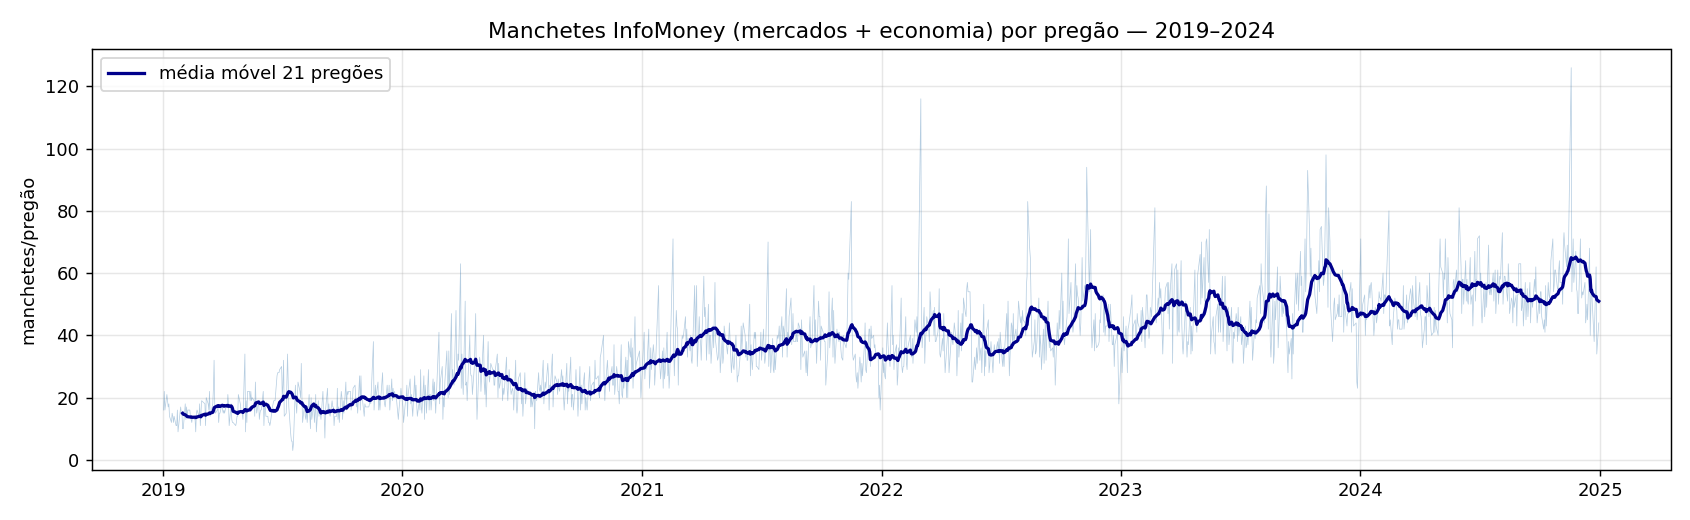
\includegraphics[width=0.48\textwidth]{manchetes_por_pregao.png}}
\caption{Manchetes coletadas por preg\~ao, 2019--2024.}
\label{fig:manchetes}
\end{figure}

\subsection{Alvo e corte temporal (anti-vazamento)}
\label{sec:antivazamento}
O alvo \'e gerado em um \'unico ponto do c\'odigo (Eq.~\eqref{eq:target}). Cada not\'icia \'e atribu\'ida ao preg\~ao cujo fechamento ela pode informar via \texttt{assign\_trading\_day}, com corte inclusivo \`as 17h (fechamento da B3): publicada at\'e 17h00 do dia $D$, atribu\'ida a $D$; depois, ao preg\~ao seguinte. Essa fun\c{c}\~ao \'e coberta por 14 testes automatizados (10 sobre o corte temporal), incluindo hor\'ario de ver\~ao hist\'orico e instantes UTC reais -- desenhados para detectar o erro cl\'assico de tratar o fuso como deslocamento fixo em vez de consultar a regra vigente na data.

\subsection{Comunicados do Copom}
Os 49 comunicados de decis\~ao de pol\'itica monet\'aria (reuni\~oes 219--267, dezembro/2018--dezembro/2024) foram obtidos via API p\'ublica de dados abertos do Banco Central. Liberados ap\'os o fechamento do preg\~ao ($\approx$18h30), s\~ao atribu\'idos ao preg\~ao seguinte pela mesma regra de corte. A reuni\~ao 219, anterior ao per\'iodo de estudo, funciona como semente de estado inicial.

\section{Metodologia}

\subsection{Vari\'aveis de pre\c{c}o}
\label{sec:features-preco}
O arquivo \texttt{features\_preco.parquet} cont\'em 18 vari\'aveis, calculadas com dados dispon\'iveis at\'e o dia $t$ para prever $t+1$: retornos defasados (lags 0--10), volatilidade realizada (5/10/21), momento (5/10/21), dist\^ancia \`a m\'edia m\'ovel (10/21), calend\'ario e duas vari\'aveis de volume relativo/varia\c{c}\~ao logar\'itmica -- nunca o n\'ivel absoluto, que carregaria tend\^encia estrutural esp\'uria. A maior correla\c{c}\~ao absoluta com o alvo \'e 0,159, consistente com aus\^encia de vazamento. O volume foi validado como sinal financeiramente plaus\'ivel: correla\c{c}\~ao com retorno absoluto de +0,18 \cite{karpoff1987} e persist\^encia estatisticamente significativa (Ljung-Box, $p\approx0$). Isoladamente, para o XGBoost, as duas vari\'aveis de volume pioram F1 (0,385 vs.\ 0,410) e MCC (0,028 vs.\ 0,040) apesar de melhorarem levemente a DA; mantivemos o conjunto de 18 vari\'aveis como definitivo para os tr\^es modelos de pre\c{c}o porque sua validade foi estabelecida por crit\'erio independente do desempenho de qualquer modelo espec\'ifico -- evitando selecionar features a posteriori -- e porque um conjunto compartilhado isola o efeito do algoritmo na compara\c{c}\~ao entre eles.

\subsection{Vari\'aveis de texto}
\textbf{BERTimbau} (\texttt{neuralmind/\allowbreak bert-base-portuguese-cased}) e \textbf{FinBERT-PT-BR} (\texttt{lucas-leme/\allowbreak FinBERT-PT-BR}) geram embeddings congelados (768 dimens\~oes) por mean-pooling mascarado por manchete, agregados por preg\~ao (m\'edia dos vetores do dia, acrescida de \texttt{n\_noticias} e dispers\~ao ao centroide). O FinBERT-PT-BR tamb\'em expõe sentimento expl\'icito (positivo/negativo/neutro) via forward oficial do classificador, agregado em quatro vari\'aveis densas por preg\~ao (\texttt{sent\_polaridade}, dispers\~ao, fra\c{c}\~oes positiva/negativa). Para redu\c{c}\~ao de dimensionalidade (768$\to k$), aplicou-se PCA ajustado \textbf{exclusivamente no treino de cada fold}, com $k\in\{8,30\}$: o BERTimbau ret\'em $\approx$45\%/69\% da vari\^ancia; o FinBERT-PT-BR, mais especializado, $\approx$86\%/92\% -- diferen\c{c}a estrutural que n\~ao se traduz em vantagem preditiva para nenhuma das duas fontes.

\subsection{Vari\'aveis do Copom}
Cada comunicado foi classificado por zero-shot (\texttt{MoritzLaurer/mDeBERTa-v3-base-mnli-xnli}) em vi\'es de aperto monet\'ario (\emph{hawkish}) versus afrouxamento (\emph{dovish}). Os comunicados (mediana 1.482 tokens) excedem o limite de 512 tokens do modelo, que trunca silenciosamente; testaram-se as janelas de in\'icio e de fim (\'ultimos 1.500 caracteres), selecionando-se a de maior correla\c{c}\~ao com a decis\~ao real de Selic: o in\'icio venceu ($r=+0{,}615$ contra $+0{,}424$), confirmando que o classificador capta vi\'es real, n\~ao ru\'ido. O score, a dire\c{c}\~ao da \'ultima decis\~ao e os dias desde a \'ultima reuni\~ao s\~ao propagados por \emph{forward-fill} di\'ario -- conven\c{c}\~ao padr\~ao em finan\c{c}as macro, segundo a qual o mercado precifica o \'ultimo vi\'es conhecido at\'e a pr\'oxima decis\~ao. O n\'ivel absoluto da Selic \'e exclu\'ido, pela mesma raz\~ao do volume (Se\c{c}\~ao~\ref{sec:features-preco}).

\subsection{Modelos}
\begin{itemize}
\item \textbf{N\'ivel 1 -- Passeio aleat\'orio.} Retorno previsto = 0; dire\c{c}\~ao = persist\^encia.
\item \textbf{N\'ivel 2 -- ARIMA/ARIMAX.} Ordem por AIC (\texttt{auto\_arima}), reajustada a cada fold, $d$=0 (ADF: $-11{,}86$, $p\approx7\times10^{-22}$); ARIMAX usa \texttt{n\_noticias}/dispers\~ao como ex\'ogenas padronizadas por fold.
\item \textbf{N\'ivel 3 -- XGBoost.} \texttt{XGBRegressor}/\texttt{Classifier}, calibra\c{c}\~ao isot\^onica via hold-out temporal interno, $N$=10 sementes.
\item \textbf{N\'ivel 4 -- LSTM (pre\c{c}o).} 1 camada, 16 unidades ocultas, dropout 0,4, lookback 21, Adam, 75 \'epocas, \texttt{StandardScaler} por fold, $N$=5 sementes, determinismo fixo.
\item \textbf{N\'ivel 5 -- LSTM (texto ou Copom).} Id\^entico ao n\'ivel 4 em arquitetura, sementes, folds e calibra\c{c}\~ao; \'unica diferen\c{c}a \'e a adi\c{c}\~ao das vari\'aveis textuais/Copom, isolando o efeito como a diferen\c{c}a frente ao n\'ivel 4.
\end{itemize}
LSTM usa \texttt{embargo=21} no walk-forward; baselines, \texttt{embargo=0}; ambos compartilham a f\'ormula $\text{fold\_size}=(n-\text{min\_train})/(n_{\text{splits}}+1)$, cobrindo janeiro/2020--fevereiro/2024 fora da amostra.

\subsection{Valida\c{c}\~ao estat\'istica e m\'etricas financeiras}
\textbf{Pesaran-Timmermann} \cite{pesaran1992} avalia se a acur\'acia direcional excede o esperado sob independ\^encia entre sinal previsto e realizado (5 folds concatenados). \textbf{Diebold-Mariano} \cite{diebold1995}, com corre\c{c}\~ao de Harvey-Leybourne-Newbold \cite{harvey1997},
\begin{equation}
DM = \frac{\bar{d}}{\sqrt{\mathrm{Var}(d)/n}}, \quad d_t = e_{1,t}^2 - e_{2,t}^2,
\label{eq:dm}
\end{equation}
compara a acur\'acia de previs\~ao entre pares de modelos. Testaram-se 13 compara\c{c}\~oes pareadas -- LSTM-pre\c{c}o vs.\ variantes de texto/Copom, e XGBoost vs.\ variantes de LSTM (interse\c{c}\~ao dos dias de teste, 185 de 206 por fold em m\'edia) --, com $p$-valores corrigidos por \textbf{Holm}. Testes DM e simula\c{c}\~oes financeiras usam a previs\~ao m\'edia entre sementes (pequeno ensemble); a DA usa o sinal da regress\~ao, enquanto F1/MCC/Brier usam a probabilidade calibrada (limiar 0,5) -- regras distintas que podem divergir em casos-limite.

Adotou-se estrat\'egia mec\^anica long/short: posi\c{c}\~ao no dia $t$ = sinal da previs\~ao; custo proporcional ao turnover. Reportam-se Sharpe anualizado e drawdown m\'aximo, sem custo (0 bps) e com custo de 5 pontos-base por opera\c{c}\~ao.

\section{Resultados}

\subsection{Diagn\'ostico de estrutura do retorno}
A Fig.~\ref{fig:acf} apresenta a autocorrela\c{c}\~ao do retorno e do retorno ao quadrado. O retorno exibe estrutura linear fraca; o retorno ao quadrado exibe \emph{clustering} de volatilidade bem mais pronunciado -- a previsibilidade dispon\'ivel na s\'erie concentra-se, majoritariamente, na vari\^ancia, n\~ao na dire\c{c}\~ao.

\begin{figure}[htbp]
\centerline{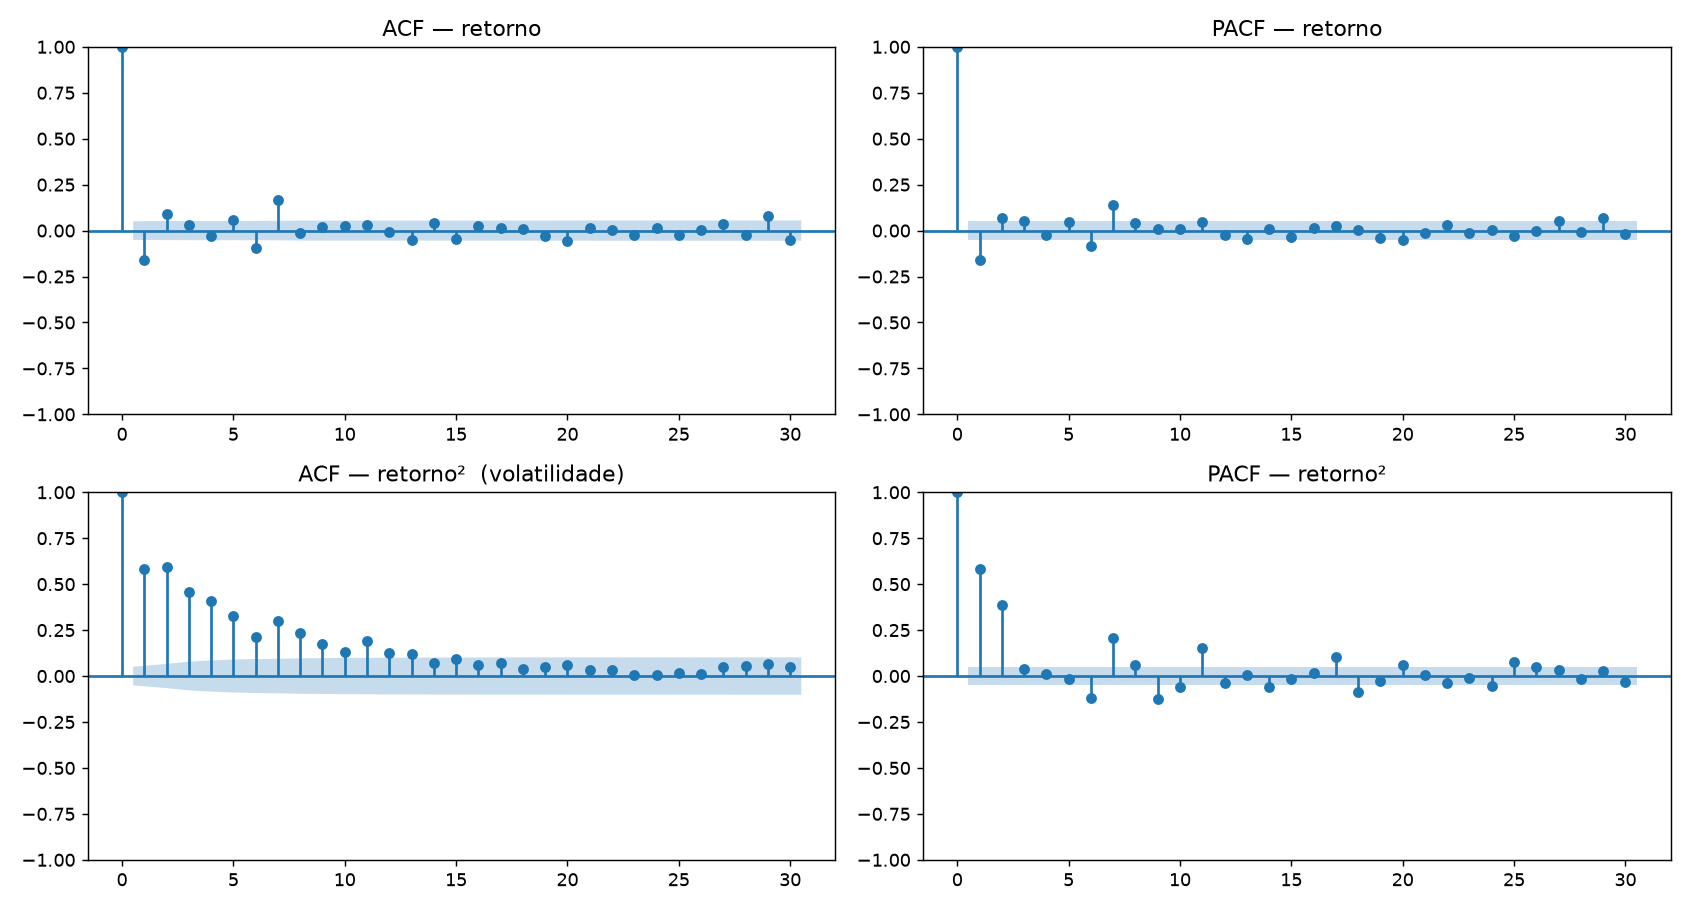
\includegraphics[width=0.48\textwidth]{acf_pacf_retorno.png}}
\caption{ACF/PACF do retorno di\'ario do Ibovespa.}
\label{fig:acf}
\end{figure}

\subsection{Tabela comparativa consolidada}
A Tabela~\ref{tab:comparativa} e a Fig.~\ref{fig:mcc} resumem os 11 modelos avaliados. Nenhum atinge signific\^ancia direcional a 5\% ap\'os corre\c{c}\~ao de Holm; o menor $p$ corrigido \'e do XGBoost (0,727). O MCC de todos os modelos situa-se dentro de um desvio-padr\~ao entre sementes em torno de zero -- vis\'ivel na Fig.~\ref{fig:mcc}, cujas barras de erro cruzam a linha zero em praticamente todos os modelos estoc\'asticos. Com $n=1030$ observa\c{c}\~oes agregadas, o intervalo de 95\% para a DA de um classificador sem habilidade direcional \'e $50\%\pm3{,}1$ p.p.; a maior DA observada (52,3\%, XGBoost) situa-se dentro dessa faixa. Os dados t\^em poder para detectar habilidade direcional a partir de $\approx$53,1\%, patamar que nenhum modelo atinge.

\begin{figure*}[htbp]
\centerline{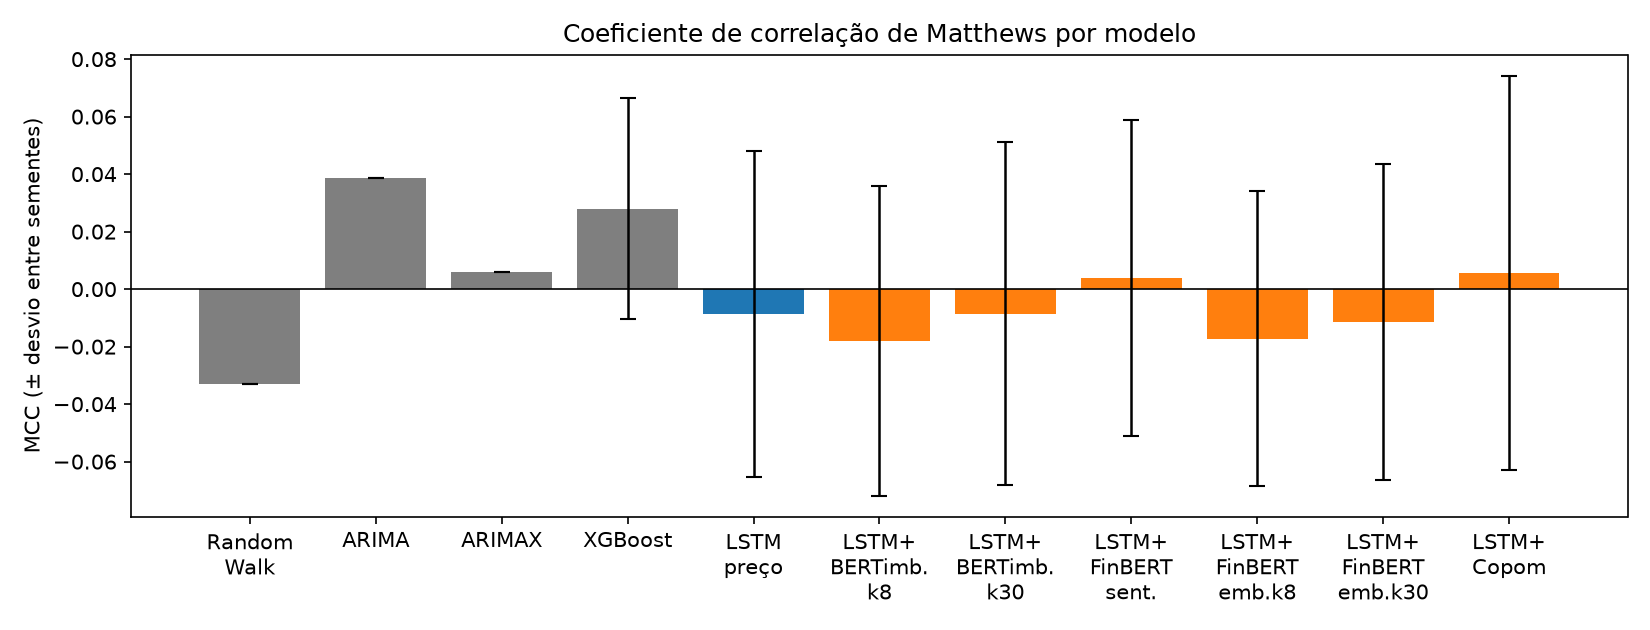
\includegraphics[width=0.85\textwidth]{fig_mcc_por_modelo.png}}
\caption{MCC por modelo, com barra de erro representando o desvio-padr\~ao entre sementes (quando aplic\'avel). Cinza: baselines determin\'isticos. Azul: LSTM apenas com pre\c{c}o. Laranja: variantes de LSTM com texto ou Copom.}
\label{fig:mcc}
\end{figure*}

\begin{table*}[htbp]
\caption{Tabela comparativa consolidada (fonte: \texttt{tabela\_comparativa\_final.csv})}
\begin{center}
\footnotesize
\begin{tabular}{lccccccc}
\toprule
\textbf{Modelo} & \textbf{MAE} & \textbf{RMSE} & \textbf{DA} & \textbf{MCC} & \textbf{MCC ($\pm$dp)} & \textbf{Brier} & \textbf{PT $p$ (Holm)} \\
\midrule
Random Walk            & 0,0116 & 0,0159 & 0,485 & $-$0,033 & --      & 0,250 & 1,000 \\
ARIMA                   & 0,0120 & 0,0166 & 0,522 & $+$0,039 & --      & --    & 1,000 \\
ARIMAX (texto linear)   & 0,0124 & 0,0181 & 0,511 & $+$0,006 & --      & --    & 1,000 \\
XGBoost (pre\c{c}o)     & 0,0117 & 0,0161 & 0,519 & $+$0,028 & 0,038   & 0,265 & 0,727 \\
LSTM (pre\c{c}o)        & 0,0127 & 0,0172 & 0,494 & $-$0,009 & 0,057   & 0,273 & 1,000 \\
LSTM + BERTimbau $k$=8  & 0,0132 & 0,0181 & 0,494 & $-$0,018 & 0,054   & 0,273 & 1,000 \\
LSTM + BERTimbau $k$=30 & 0,0133 & 0,0178 & 0,508 & $-$0,009 & 0,060   & 0,265 & 1,000 \\
LSTM + FinBERT sent.    & 0,0136 & 0,0182 & 0,498 & $+$0,004 & 0,055   & 0,273 & 1,000 \\
LSTM + FinBERT emb. $k$=8  & 0,0136 & 0,0183 & 0,491 & $-$0,017 & 0,051 & 0,276 & 1,000 \\
LSTM + FinBERT emb. $k$=30 & 0,0131 & 0,0178 & 0,502 & $-$0,012 & 0,055 & 0,271 & 1,000 \\
LSTM + Copom            & 0,0140 & 0,0186 & 0,507 & $+$0,006 & 0,069   & 0,263 & 1,000 \\
\bottomrule
\end{tabular}
\label{tab:comparativa}
\end{center}
\end{table*}

\subsection{Testes pareados (Diebold-Mariano)}
Das 13 compara\c{c}\~oes pareadas testadas, 5 permanecem significativas a 5\% ap\'os corre\c{c}\~ao de Holm (Tabela~\ref{tab:dm}), incluindo XGBoost vs.\ LSTM+Copom. Em nenhuma delas a adi\c{c}\~ao de texto ou Copom reduz o erro de forma significativa; quando h\'a signific\^ancia, aponta sempre na dire\c{c}\~ao oposta -- o modelo mais simples vence.

\begin{table}[H]
\caption{Compara\c{c}\~oes DM significativas ap\'os corre\c{c}\~ao de Holm}
\begin{center}
\footnotesize
\resizebox{\columnwidth}{!}{%
\begin{tabular}{lcccc}
\toprule
\textbf{Compara\c{c}\~ao} & \textbf{DM} & \textbf{$\bar{d}$} & \textbf{$p$ (Holm)} & \textbf{Dire\c{c}\~ao} \\
\midrule
pre\c{c}o vs.\ FinBERT-sent.     & $-3{,}12$ & $-0{,}00004$ & 0,019 & texto piora \\
XGB vs.\ BERTimbau $k$=30    & $-3{,}53$ & $-0{,}00004$ & 0,005 & XGB melhor \\
XGB vs.\ FinBERT-sent.       & $-3{,}91$ & $-0{,}00006$ & 0,001 & XGB melhor \\
XGB vs.\ FinBERT emb.\ $k$=30 & $-3{,}22$ & $-0{,}00003$ & 0,015 & XGB melhor \\
XGB vs.\ Copom               & $-2{,}79$ & $-0{,}00005$ & 0,048 & XGB melhor \\
\bottomrule
\end{tabular}%
}
\label{tab:dm}
\end{center}
\end{table}

Esse achado corrobora, com respaldo estat\'istico formal, um padr\~ao qualitativo j\'a observ\'avel na progress\~ao de complexidade: aumentar a sofistica\c{c}\~ao do modelo (RW$\to$ARIMA$\to$XGBoost$\to$LSTM) n\~ao melhora a previs\~ao; em v\'arias compara\c{c}\~oes diretas, o modelo mais simples \'e mensuravelmente superior. Duas ressalvas: a fam\'ilia de 13 testes foi definida pela estrutura do desenho experimental, n\~ao registrada previamente -- a corre\c{c}\~ao de Holm protege contra infla\c{c}\~ao de falso-positivo \emph{dentro} dessa fam\'ilia, mas n\~ao contra compara\c{c}\~oes n\~ao declaradas mais amplas; e, mais relevante, signific\^ancia estat\'istica n\~ao implica relev\^ancia econ\^omica -- as diferen\c{c}as de erro subjacentes aos 5 resultados significativos s\~ao da ordem de $10^{-5}$, detect\'aveis por $n\approx1030$ conferir poder estat\'istico, n\~ao por magnitude economicamente relevante (Se\c{c}\~ao~\ref{sec:financeiro-discussao}).

\subsection{Robustez: defasagem temporal, lookback e agrega\c{c}\~ao por rec\^encia}
\label{sec:robustez}
Substituir o texto do dia $D$ pelo do dia anterior ($D-1$) no LSTM+BERTimbau $k$=8 n\~ao altera o quadro geral -- MCC de $-0{,}016\pm0{,}054$, valor intermedi\'ario entre o modelo s\'o-pre\c{c}o ($-0{,}009$) e o texto de $D$ ($-0{,}018\pm0{,}054$). A Tabela~\ref{tab:lookback} varia o lookback em $\{1,3,5,10,21\}$: em nenhuma janela o MCC ultrapassa o intervalo de um desvio-padr\~ao entre sementes em torno de zero -- o resultado nulo n\~ao \'e artefato da escolha de 21 dias. Testou-se ainda substituir a m\'edia diária de manchetes pela \'unica manchete mais recente antes do corte (agrega\c{c}\~ao por rec\^encia, motivada pelo achado de que o sinal textual \'e contempor\^aneo -- Se\c{c}\~ao~\ref{sec:achado}): MCC de $-0{,}023\pm0{,}052$, dentro do mesmo ru\'ido da m\'edia do dia, sem eleva\c{c}\~ao da correla\c{c}\~ao preditiva ($|r|$ m\'aximo $=0{,}057$) -- concentrar-se na informa\c{c}\~ao mais recente do dia tamb\'em n\~ao destrava sinal.

\begin{table}[H]
\caption{MCC por janela de lookback (embargo = lookback em cada linha)}
\begin{center}
\footnotesize
\begin{tabular}{ccc}
\toprule
\textbf{Lookback} & \textbf{MCC s\'o-pre\c{c}o} & \textbf{MCC + BERTimbau $k$=8} \\
\midrule
1  & $-0{,}014\pm0{,}068$ & $+0{,}001\pm0{,}060$ \\
3  & $-0{,}006\pm0{,}042$ & $-0{,}021\pm0{,}053$ \\
5  & $-0{,}003\pm0{,}043$ & $-0{,}012\pm0{,}052$ \\
10 & $+0{,}005\pm0{,}045$ & $-0{,}006\pm0{,}055$ \\
21 & $-0{,}009\pm0{,}057$ & $-0{,}018\pm0{,}054$ \\
\bottomrule
\end{tabular}
\label{tab:lookback}
\end{center}
\end{table}

\subsection{Robustez: anisotropia dos embeddings e qualidade textual}
\label{sec:anisotropia}
Embeddings de BERT s\~ao conhecidamente anisotr\'opicos \cite{ethayarajh2019}: textos sem rela\c{c}\~ao sem\^antica exibem similaridade de cosseno bem acima de zero, pois parte da vari\^ancia do espa\c{c}o vetorial concentra-se numa dire\c{c}\~ao gen\'erica n\~ao-informativa. A similaridade m\'edia entre pares aleat\'orios de manchetes \'e $0{,}659$ (esperar-se-ia $\approx0$ sob isotropia), confirmando anisotropia relevante. \emph{Whitening} explorat\'orio (decorrela\c{c}\~ao e equaliza\c{c}\~ao de vari\^ancia, ao molde de BERT-flow) eleva e estabiliza a correla\c{c}\~ao \emph{contempor\^anea} do BERTimbau (de $0{,}03$--$0{,}09$ para $0{,}067$--$0{,}077$); para o FinBERT, j\'a especializado, a correla\c{c}\~ao contempor\^anea \'e alta mesmo nos embeddings crus ($0{,}215$) e n\~ao se beneficia da corre\c{c}\~ao. Em ambas as fontes, contudo, a correla\c{c}\~ao \textbf{preditiva} permanece na faixa de ru\'ido para todo $k\in\{8,30,100,300\}$ testado (Tabela~\ref{tab:anisotropia}); teste de permuta\c{c}\~ao (500 repeti\c{c}\~oes) confirma que o maior valor observado ($r=0{,}090$) \'e indistingu\'ivel de ru\'ido ($p=0{,}178$).

\begin{table}[H]
\caption{Correla\c{c}\~ao m\'axima ($|r|$) entre componentes e o alvo, cru vs.\ whitened ($k=300$)}
\begin{center}
\footnotesize
\begin{tabular}{lcccc}
\toprule
\textbf{Fonte} & \multicolumn{2}{c}{\textbf{Preditivo}} & \multicolumn{2}{c}{\textbf{Contempor\^aneo}} \\
 & cru & whitened & cru & whitened \\
\midrule
BERTimbau & 0,085 & 0,090 & 0,088 & 0,068 \\
FinBERT   & 0,082 & 0,079 & 0,215 & 0,189 \\
\bottomrule
\end{tabular}
\label{tab:anisotropia}
\end{center}
\end{table}

Remo\c{c}\~ao de manchetes-template recorrentes (1,5\% do corpus) e isolamento de linguagem prospectiva (9,6\%) versus retrospectiva (0,4\%) tamb\'em n\~ao produziram correla\c{c}\~ao preditiva distingu\'ivel de ru\'ido ($p\in\{0{,}29$--$0{,}87\}$ em todos os casos).

Testou-se ainda hip\'otese mais radical: seria a pr\'opria representa\c{c}\~ao densa, e n\~ao a anisotropia, o fator limitante? A literatura recente de embeddings financeiros documenta que um \emph{bag-of-words} (BoW) simples supera embeddings densos em similaridade sem\^antica financeira \cite{tangyang2025}. Substituiu-se o embedding do BERTimbau por TF-IDF do texto do dia reduzido via SVD truncada (an\'alogo esparso ao PCA), vocabul\'ario e SVD ajustados s\'o no treino de cada fold (Tabela~\ref{tab:bow}): o MCC esparso \'e indistingu\'ivel do denso e de zero em ambos os $k$ testados. O achado da literatura n\~ao se replica aqui.

\begin{table}[H]
\caption{MCC preditivo: representa\c{c}\~ao densa vs.\ esparsa}
\begin{center}
\footnotesize
\begin{tabular}{lcc}
\toprule
\textbf{Representa\c{c}\~ao} & \textbf{MCC ($k$=8)} & \textbf{MCC ($k$=30)} \\
\midrule
BERTimbau (denso)    & $-0{,}018\pm0{,}054$ & $-0{,}009\pm0{,}060$ \\
BoW/TF-IDF (esparso) & $-0{,}021\pm0{,}063$ & $-0{,}016\pm0{,}052$ \\
\bottomrule
\end{tabular}
\label{tab:bow}
\end{center}
\end{table}

O resultado nulo mostra-se, portanto, robusto tanto \`a anisotropia dos embeddings quanto a interven\c{c}\~oes razo\'aveis de limpeza textual e \`a substitui\c{c}\~ao da representa\c{c}\~ao densa por uma esparsa.

\subsection{Robustez: corpo completo das mat\'erias}
\label{sec:corpo-completo}
A an\'alise anterior usa exclusivamente a manchete de cada mat\'eria (Se\c{c}\~ao~\ref{sec:limitacoes}). Recoletou-se o corpo completo de 56.819 mat\'erias (98,6\% do corpus; mediana de 2.584 caracteres, contra dezenas na manchete) e retreinou-se todas as variantes de texto sob protocolo id\^entico, com embeddings extra\'idos a 512 tokens (limite do modelo, contra 64 usados para manchetes). Os $\Delta$MCC frente \`a manchete ficam entre $-0{,}002$ e $+0{,}015$ para as cinco variantes de texto -- muito abaixo do desvio-padr\~ao entre sementes ($0{,}04$--$0{,}07$). O teste de Pesaran-Timmermann pooled permanece n\~ao significativo para os 11 modelos ap\'os Holm, e o padr\~ao qualitativo dos testes DM se mant\'em: XGBoost ocasionalmente supera variantes de LSTM+texto, nunca o inverso. Conclui-se que ampliar o texto dispon\'ivel em cerca de trinta vezes n\~ao desloca MCC, acur\'acia direcional ou signific\^ancia estat\'istica de forma percept\'ivel -- refor\c{c}ando a explica\c{c}\~ao mecan\'istica da Se\c{c}\~ao~\ref{sec:achado} (sinal contempor\^aneo, n\~ao preditivo) como causa mais prov\'avel do resultado nulo do que a insufici\^encia de texto dispon\'ivel. Testou-se ainda se o pr\'oprio truncamento em 512 tokens do corpo completo escondia sinal: dividindo cada mat\'eria em blocos de at\'e 512 tokens (\emph{chunking}, 123.570 blocos ao todo) e agregando por m\'edia, o MCC permanece na mesma faixa de ru\'ido (ex.: BERTimbau $k$=8: $-0{,}015$ com \emph{chunking} vs.\ $-0{,}003$ truncado vs.\ $-0{,}018$ manchete) -- nem o escopo (manchete vs.\ corpo) nem o comprimento de contexto explicam o resultado nulo.

\subsection{Sentimento reativo versus sentimento preditivo}
\label{sec:achado}
A correla\c{c}\~ao entre o sentimento do FinBERT-PT-BR e o retorno depende substancialmente da dire\c{c}\~ao temporal (Fig.~\ref{fig:sentimento}): contempor\^anea (dia $t$ vs.\ retorno de $t$), $r=+0{,}201$; preditiva (dia $t$ vs.\ retorno de D+1, o alvo), $r=-0{,}039$. Como as duas correla\c{c}\~oes compartilham a vari\'avel de sentimento e usam retornos adjacentes da mesma s\'erie (n\~ao independentes), testou-se a diferen\c{c}a via bootstrap dependente ($B=20\,000$): $p=0{,}0001$, significativa a 5\% mesmo ap\'os corre\c{c}\~ao de Holm para as 4 vari\'aveis de sentimento testadas.

\begin{figure}[htbp]
\centerline{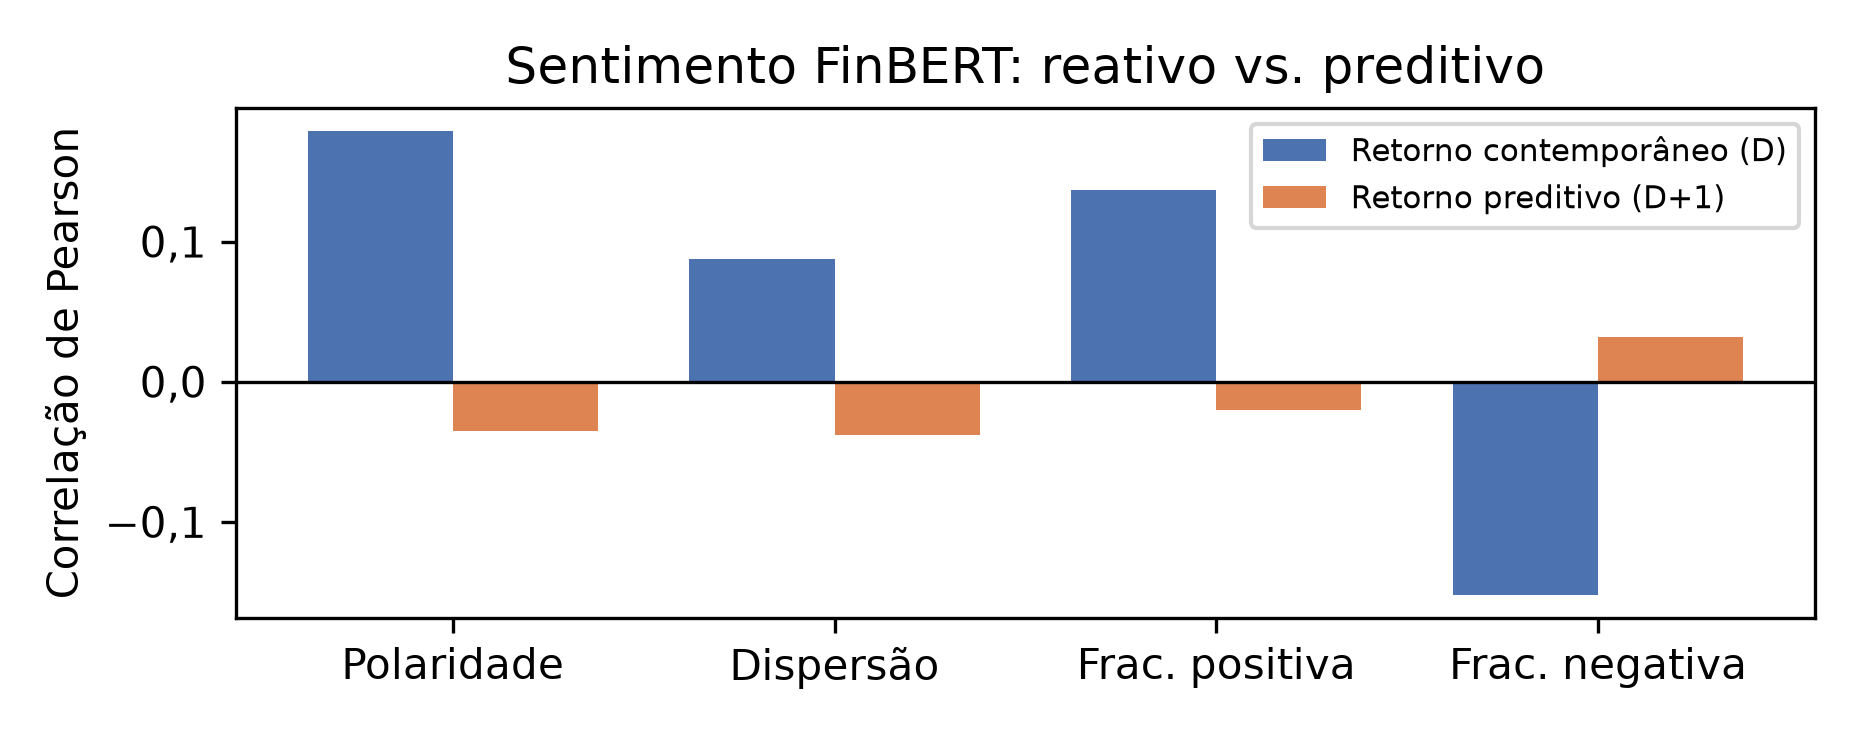
\includegraphics[width=0.48\textwidth]{fig_sentimento_reativo.png}}
\caption{Correla\c{c}\~ao das vari\'aveis de sentimento FinBERT com o retorno contempor\^aneo (D) versus o retorno preditivo (D+1, o alvo).}
\label{fig:sentimento}
\end{figure}

As quatro vari\'aveis de sentimento agregado t\^em correla\c{c}\~ao preditiva entre $-0{,}04$ e $+0{,}03$ -- indistingu\'ivel de zero --, enquanto a correla\c{c}\~ao contempor\^anea de \texttt{sent\_polaridade} \'e cerca de cinco vezes maior. Essa assimetria constitui a explica\c{c}\~ao mecan\'istica proposta neste trabalho para a aus\^encia de ganho preditivo do texto em todas as arquiteturas testadas: as not\'icias financeiras descrevem com fidelidade o que j\'a ocorreu no mercado no mesmo dia, mas n\~ao antecipam o que ocorrer\'a no dia seguinte -- consistente com a hip\'otese de efici\^encia informacional de mercado. O FinBERT-PT-BR utilizado exibe vi\'es para sentimento negativo (53\% das manchetes, contra 21\% positivas, em per\'iodo de alta acumulada do \'indice); a hip\'otese inicial de que isso decorreria de confus\~ao de vocabul\'ario t\'ecnico foi testada e n\~ao confirmada na Se\c{c}\~ao~\ref{sec:limitacoes} (um modelo gen\'erico independente \'e \emph{ainda mais} negativo, sugerindo estilo editorial, n\~ao o modelo espec\'ifico). Em todo caso, como a correla\c{c}\~ao preditiva foi calculada sobre a polaridade cont\'inua, e n\~ao sobre a classe discreta, esse vi\'es n\~ao explica o resultado nulo.

\subsection{M\'etricas financeiras}
\label{sec:financeiro-discussao}
A Tabela~\ref{tab:financeiro} mostra que, sem custo de transa\c{c}\~ao, 4 dos 11 modelos exibem Sharpe bruto positivo. Sob custo realista de 5 pontos-base por opera\c{c}\~ao, \textbf{dez dos onze modelos apresentam Sharpe negativo ou nulo}, inclusive o LSTM+BERTimbau $k$=30 (de $+0{,}175$ para $-0{,}019$). A \'unica exce\c{c}\~ao \'e o LSTM+Copom (Sharpe l\'iquido $+0{,}42$), que exige leitura criteriosa: retorno m\'edio di\'ario estatisticamente indistingu\'ivel de zero ($t=0{,}86$, $p\approx0{,}39$); desempenho inst\'avel entre folds ($+0{,}84$, $+1{,}78$, $-1{,}69$, $+0{,}57$, $+0{,}18$; perda de 23,6\% no terceiro); e trata-se do m\'aximo entre 11 estrat\'egias derivadas de modelos sem habilidade direcional detect\'avel (PT $p=0{,}27$ sem corre\c{c}\~ao; MCC $+0{,}006\pm0{,}069$) -- o m\'aximo de v\'arios modelos nulos tende a parecer positivo por efeito de sele\c{c}\~ao, n\~ao capacidade preditiva gen\'uina.

\begin{table*}[htbp]
\caption{M\'etricas financeiras (fonte: \texttt{metricas\_financeiras.csv}). Linha RW: previs\~ao de regress\~ao \'e zero, estrat\'egia nunca opera (piso trivial).}
\begin{center}
\footnotesize
\begin{tabular}{lcccc}
\toprule
\textbf{Modelo} & \textbf{Sharpe (0 bps)} & \textbf{Sharpe (5 bps)} & \textbf{MaxDD (5 bps)} & \textbf{N.\ trades} \\
\midrule
Buy-and-hold (refer\^encia) & 0,091 & --      & $-46{,}8\%$ & -- \\
Random Walk                & 0,000 & 0,000   & $0{,}0\%$   & 0 \\
ARIMA                      & $-0{,}035$ & $-0{,}445$ & $-45{,}2\%$ & 469 \\
ARIMAX                     & $+0{,}149$ & $-0{,}258$ & $-34{,}7\%$ & 467 \\
XGBoost                    & $-0{,}083$ & $-0{,}406$ & $-50{,}6\%$ & 371 \\
LSTM (pre\c{c}o)           & $-0{,}277$ & $-0{,}570$ & $-55{,}3\%$ & 335 \\
LSTM + BERTimbau $k$=8     & $-1{,}017$ & $-1{,}251$ & $-76{,}2\%$ & 267 \\
LSTM + BERTimbau $k$=30    & $\mathbf{+0{,}175}$ & $-0{,}019$ & $-41{,}1\%$ & 221 \\
LSTM + FinBERT sent.       & $-0{,}308$ & $-0{,}584$ & $-60{,}8\%$ & 316 \\
LSTM + FinBERT emb.\ $k$=8  & $+0{,}063$ & $-0{,}196$ & $-38{,}9\%$ & 296 \\
LSTM + FinBERT emb.\ $k$=30 & $-0{,}312$ & $-0{,}537$ & $-58{,}1\%$ & 258 \\
LSTM + Copom                & $+0{,}688$ & $+0{,}424$ & $-37{,}7\%$ & 301 \\
\bottomrule
\end{tabular}
\label{tab:financeiro}
\end{center}
\end{table*}

\begin{figure*}[htbp]
\centerline{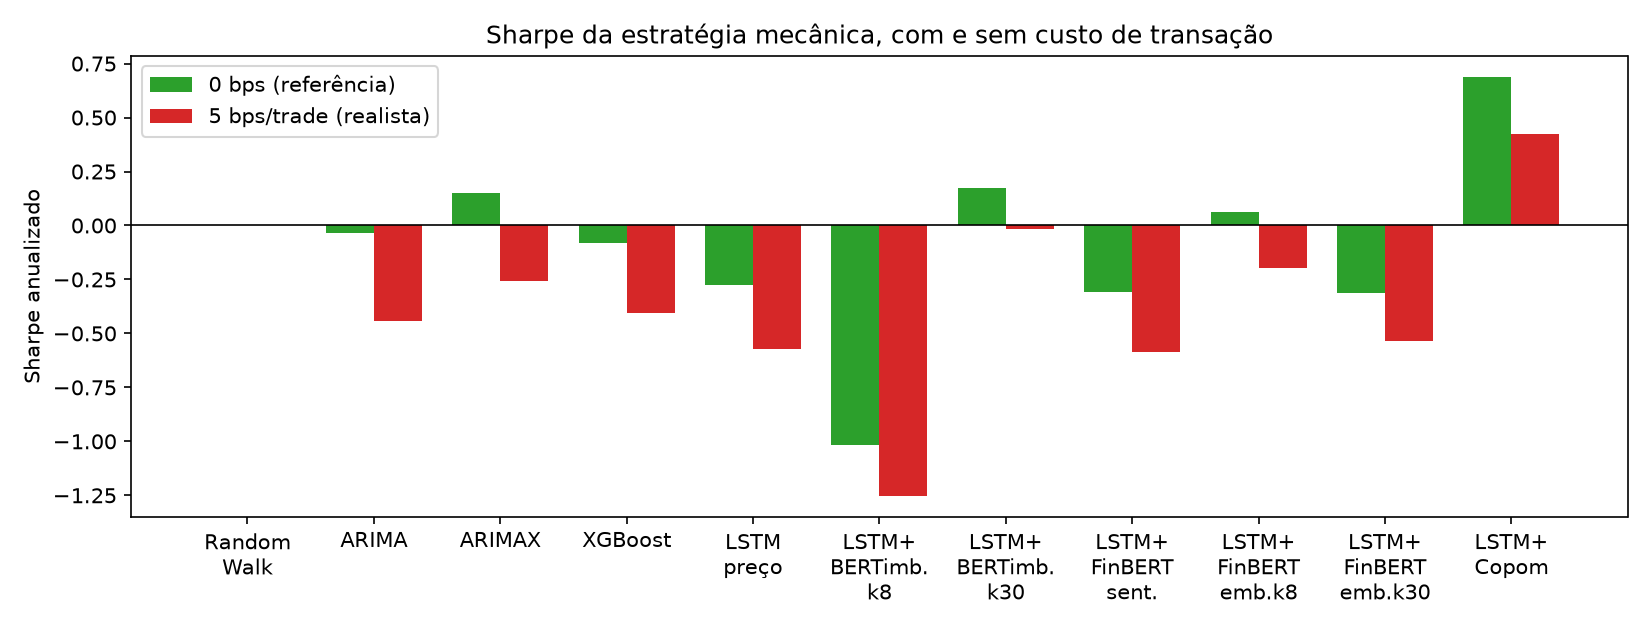
\includegraphics[width=0.85\textwidth]{fig_sharpe_custo.png}}
\caption{Sharpe anualizado por modelo, sem custo de transa\c{c}\~ao (0 bps) e com custo realista (5 bps/trade). Dez dos onze modelos ficam negativos ou pr\'oximos de zero sob custo; a exce\c{c}\~ao (LSTM+Copom) \'e estatisticamente indistingu\'ivel de zero e inst\'avel entre folds.}
\label{fig:sharpe}
\end{figure*}

O Random Walk, por nunca assumir posi\c{c}\~ao, constitui piso trivial de compara\c{c}\~ao. Esse conjunto de resultados, ilustrado na Fig.~\ref{fig:sharpe}, corrobora, sob m\'etrica de utilidade econ\^omica direta, a conclus\~ao dos testes estat\'isticos de acur\'acia: nenhum modelo produz vantagem operacionaliz\'avel.

\section{Discuss\~ao}

Os resultados convergem, sob tr\^es perspectivas independentes -- magnitude do erro, habilidade direcional formal e utilidade econ\^omica --, para uma conclus\~ao \'unica: nenhum modelo, com ou sem texto, prev\^e o retorno di\'ario do Ibovespa de forma estatisticamente distingu\'ivel do acaso.

O achado mais relevante n\~ao \'e a aus\^encia de sinal em si, mas a \emph{explica\c{c}\~ao mecan\'istica} (Se\c{c}\~ao~\ref{sec:achado}): o texto financeiro em portugu\^es carrega sinal gen\'uino sobre o mercado, por\'em esse sinal \'e \textbf{contempor\^aneo}, n\~ao \textbf{preditivo}. Esse aspecto distingue este trabalho de resultados nulos n\~ao explicados e de trabalhos que reportam ganhos sem controle adequado de vazamento temporal, problema recorrente na literatura de FinBERT-LSTM discutida na Se\c{c}\~ao~\ref{sec:relacionados}.

O sinal do Copom estende esse padr\~ao a uma fonte estruturalmente distinta: evento raro (49 reuni\~oes em 6 anos, contra 57.611 manchetes), de car\'ater oficial, com vi\'es diretamente verific\'avel contra a decis\~ao real de Selic ($r=+0{,}615$). O classificador \'e eficaz, mas o sinal assim capturado tampouco antecipa o retorno de D+1. Informa\c{c}\~ao p\'ublica relevante, qualquer que seja sua fonte, parece j\'a estar precificada no fechamento do dia em que se torna conhecida.

A superioridade estatisticamente significativa do XGBoost em rela\c{c}\~ao a diversas variantes de LSTM n\~ao significa que o XGBoost preveja o mercado -- seu MCC de $+0{,}028\pm0{,}038$ tamb\'em n\~ao \'e distingu\'ivel de zero --, mas que, entre modelos igualmente desprovidos de habilidade preditiva real, os mais simples produzem erros de magnitude menor e mais est\'avel, argumento favor\'avel \`a pars\^imonia mesmo quando nenhum modelo alcan\c{c}a sucesso preditivo. Registra-se ainda que o MCC do passeio aleat\'orio direcional (persist\^encia) \'e \emph{negativo} ($-0{,}033$), sugerindo leve revers\~ao \`a m\'edia de curt\'issimo prazo -- estrutura fraca que nenhuma arquitetura testada converteu em habilidade preditiva significativa, refor\c{c}ando a leitura de efici\^encia informacional. Esse grau de efici\^encia \'e compat\'ivel com a evolu\c{c}\~ao hist\'orica documentada para a Bovespa: \cite{torres2002} rejeitaram passeio aleat\'orio na s\'erie di\'aria/semanal entre 1986--1998, mas com grau de rejei\c{c}\~ao decrescente ao longo da amostra, sobretudo ap\'os o Plano Real -- tend\^encia com a qual a estrutura linear fraca (n\~ao ausente) desta amostra, duas d\'ecadas mais recente, \'e consistente.

\section{Limita\c{c}\~oes}
\label{sec:limitacoes}

\begin{itemize}
\item \textbf{Frequ\^encia di\'aria.} Fechamentos di\'arios podem subestimar a velocidade real de incorpora\c{c}\~ao de not\'icias ao pre\c{c}o.
\item \textbf{Vi\'es de classifica\c{c}\~ao do FinBERT-PT-BR.} Sobrerrepresenta\c{c}\~ao de sentimento negativo (53\% vs.\ 21\% positivo) em per\'iodo de alta. Comparado a um modelo independente, sem ajuste financeiro (\texttt{nlptown/\allowbreak bert-base-multilingual-uncased-sentiment}), sobre o mesmo corpus: o modelo gen\'erico classifica fra\c{c}\~ao \textbf{maior} como negativa (67,7\%) -- contr\'ario \`a hip\'otese de vi\'es espec\'ifico do FinBERT-PT-BR, sugerindo estilo editorial das manchetes, n\~ao confus\~ao de vocabul\'ario t\'ecnico. Correla\c{c}\~ao entre polaridades dos dois modelos: $r=+0{,}359$; correla\c{c}\~ao preditiva do modelo alternativo tamb\'em nula ($r=+0{,}011$ vs.\ $+0{,}075$ contempor\^anea) -- mesmo padr\~ao reativo, via independente.
\item \textbf{Escopo textual.} O resultado nulo replica-se tanto com o corpo completo quanto com \emph{chunking} cobrindo o artigo inteiro sem truncamento (Se\c{c}\~ao~\ref{sec:corpo-completo}) -- nem o escopo (manchete vs.\ corpo) nem o comprimento de contexto dispon\'ivel ao modelo explicam a aus\^encia de sinal preditivo.
\item \textbf{Cobertura editorial \'unica.} Corpus restrito a um \'unico ve\'iculo (InfoMoney); vi\'eses editoriais espec\'ificos n\~ao foram comparados a outras fontes.
\item \textbf{Edi\c{c}\~ao de mat\'erias ap\'os a publica\c{c}\~ao original.} 4,3\% das mat\'erias foram editadas mais de 24h ap\'os a publica\c{c}\~ao, e 2,6\% mais de 7 dias depois -- risco real, ainda que reduzido, de diverg\^encia com o texto publicado em tempo real.
\item \textbf{Recorr\^encia vs.\ capacidade.} MLP raso (1 camada, 32 unidades, mesmo regime de treino da LSTM) sobre a janela achatada obteve MCC $-0{,}004\pm0{,}046$, indistingu\'ivel do MCC da LSTM ($-0{,}009\pm0{,}057$) -- a recorr\^encia n\~ao agrega vantagem detect\'avel sobre um MLP raso.
\item \textbf{Efici\^encia em dado pequeno.} O mesmo texto acoplado ao XGBoost (mais eficiente que a LSTM em dado pequeno) tampouco supera o XGBoost s\'o-pre\c{c}o ($+0{,}028\pm0{,}038$) em nenhuma das 5 vari\'aveis textuais testadas -- o resultado nulo n\~ao decorre da escolha de arquitetura.
\item \textbf{Interpreta\c{c}\~ao de componentes de PCA.} PCA (k=8) ajustado sobre a s\'erie completa, s\'o para diagn\'ostico: os componentes de maior vari\^ancia correlacionam-se principalmente com volume editorial ($n\_noticias$, $r=+0{,}43$) e secundariamente com polaridade de sentimento, mas nenhum com o retorno contempor\^aneo ou de D+1 ($|r|\leq0{,}04$ em todos).
\item \textbf{Migra\c{c}\~ao de ambiente computacional.} Resultados originalmente produzidos em GPU T4 (Colab), reproduzidos localmente em RTX 3070 dentro da varia\c{c}\~ao esperada entre sementes, sem altera\c{c}\~ao de conclus\~oes qualitativas.
\item \textbf{Estrat\'egia financeira estilizada.} Avalia\c{c}\~ao de Sharpe/drawdown emprega estrat\'egia mec\^anica simples, sem dimensionamento de posi\c{c}\~ao, \emph{stop-loss} ou custo de financiamento.
\item \textbf{Escolha dos modelos de embedding.} BERTimbau e FinBERT-PT-BR n\~ao foram comparados contra alternativas mais recentes de representa\c{c}\~ao textual em portugu\^es; um sinal nulo com esses dois modelos n\~ao descarta que um embedding mais moderno capture algo diferente.
\end{itemize}

\section{Conclus\~ao}

Sob protocolo de valida\c{c}\~ao walk-forward rigoroso -- embargo temporal apropriado, ajuste de todo componente dependente de dados exclusivamente no treino de cada fold, avalia\c{c}\~ao multi-semente e testes formais de signific\^ancia com corre\c{c}\~ao para m\'ultiplas compara\c{c}\~oes --, nenhum modelo testado, com ou sem embeddings de not\'icias financeiras em portugu\^es ou sinal de pol\'itica monet\'aria do Copom, prev\^e o retorno di\'ario do Ibovespa de forma estatisticamente distingu\'ivel do acaso. O sinal textual presente nas manchetes financeiras \'e gen\'uino, por\'em reativo: descreve o retorno do pr\'oprio dia com correla\c{c}\~ao de $+0{,}20$, e n\~ao o retorno do dia seguinte, cuja correla\c{c}\~ao com o sentimento \'e estatisticamente nula.

Trata-se de resultado nulo obtido com rigor metodol\'ogico, e n\~ao de limita\c{c}\~ao de implementa\c{c}\~ao. Demonstrar de forma controlada e reprodut\'ivel que um canal de informa\c{c}\~ao amplamente considerado \'util n\~ao produz vantagem preditiva mensur\'avel, e explicar \emph{por que} esse resultado ocorre, constitui, em si, contribui\c{c}\~ao cient\'ifica v\'alida.

\section*{Reprodutibilidade}
Todo o c\'odigo-fonte -- notebooks, scripts de coleta e o m\'odulo \texttt{utils/tcc\_utils.py} -- est\'a publicado no reposit\'orio do projeto no GitHub, com instru\c{c}\~oes em \texttt{README.md} e ambiente fixado em \texttt{requirements.txt}. Dados brutos, vari\'aveis derivadas e resultados podem ser integralmente reconstitu\'idos a partir desse c\'odigo; por seu volume, n\~ao s\~ao distribu\'idos no mesmo reposit\'orio, mas podem ser disponibilizados sob solicita\c{c}\~ao. A su\'ite \texttt{test\_tcc\_utils.py} (14 casos, corte temporal, hor\'ario de ver\~ao, embargo e gera\c{c}\~ao do alvo) verifica formalmente as garantias anti-vazamento da Se\c{c}\~ao~\ref{sec:antivazamento}.

\begin{thebibliography}{00}
\bibitem{araci2019finbert} D. Araci, ``FinBERT: Financial Sentiment Analysis with Pre-trained Language Models,'' \emph{arXiv preprint arXiv:1908.10063}, 2019.
\bibitem{diebold1995} F. X. Diebold and R. S. Mariano, ``Comparing Predictive Accuracy,'' \emph{Journal of Business \& Economic Statistics}, vol. 13, no. 3, pp. 253--263, 1995.
\bibitem{harvey1997} D. Harvey, S. Leybourne, and P. Newbold, ``Testing the Equality of Prediction Mean Squared Errors,'' \emph{International Journal of Forecasting}, vol. 13, no. 2, pp. 281--291, 1997.
\bibitem{karpoff1987} J. M. Karpoff, ``The Relation Between Price Changes and Trading Volume: A Survey,'' \emph{Journal of Financial and Quantitative Analysis}, vol. 22, no. 1, pp. 109--126, 1987.
\bibitem{pesaran1992} M. H. Pesaran and A. Timmermann, ``A Simple Nonparametric Test of Predictive Performance,'' \emph{Journal of Business \& Economic Statistics}, vol. 10, no. 4, pp. 461--465, 1992.
\bibitem{gu2024finbertlstm} W. Gu, Y. Zhong, S. Li, C. Wei, L. Dong, Z. Wang, and C. Yan, ``Predicting Stock Prices with FinBERT-LSTM: Integrating News Sentiment Analysis,'' in \emph{Proc. 8th Int. Conf. on Cloud and Big Data Computing (ICCBDC)}, Oxford, UK, 2024. DOI: 10.1145/3694860.3694870.
\bibitem{dahal2023comparative} K. R. Dahal, N. R. Pokhrel, S. Gaire, S. Mahatara, R. P. Joshi, A. Gupta, H. R. Banjade, and J. Joshi, ``A comparative study on effect of news sentiment on stock price prediction with deep learning architecture,'' \emph{PLOS ONE}, vol. 18, no. 4, e0284695, 2023.
\bibitem{ethayarajh2019} K. Ethayarajh, ``How Contextual are Contextualized Word Representations? Comparing the Geometry of BERT, ELMo, and GPT-2 Embeddings,'' in \emph{Proc. 2019 Conf. on Empirical Methods in Natural Language Processing and 9th Int. Joint Conf. on Natural Language Processing (EMNLP-IJCNLP)}, pp. 55--65, 2019.
\bibitem{loughran2011} T. Loughran and B. McDonald, ``When Is a Liability Not a Liability? Textual Analysis, Dictionaries, and 10-Ks,'' \emph{The Journal of Finance}, vol. 66, no. 1, pp. 35--65, 2011.
\bibitem{gukellyxiu2020} S. Gu, B. Kelly, and D. Xiu, ``Empirical Asset Pricing via Machine Learning,'' \emph{The Review of Financial Studies}, vol. 33, no. 5, pp. 2223--2273, 2020.
\bibitem{sirignanocont2019} J. Sirignano and R. Cont, ``Universal features of price formation in financial markets: perspectives from Deep Learning,'' \emph{Quantitative Finance}, vol. 19, no. 9, pp. 1449--1459, 2019.
\bibitem{torres2002} R. Torres, M. Bonomo, and C. Fernandes, ``A Aleatoriedade do Passeio na Bovespa: Testando a Efici\^encia do Mercado Acion\'ario Brasileiro,'' \emph{Revista Brasileira de Economia}, vol. 56, no. 2, 2002.
\bibitem{tangyang2025} Y. Tang and Y. Yang, ``FinMTEB: Finance Massive Text Embedding Benchmark,'' in \emph{Proc. 2025 Conf. on Empirical Methods in Natural Language Processing (EMNLP)}, 2025.
\end{thebibliography}

\end{document}
